\section{Busca Ternária}

\begin{frame}[fragile]{Motivação}

    \begin{itemize}
        \item A busca ternária também utiliza a divisão e conquista para reduzir significativamente
            o espaço de busca a cada iteração do algoritmo

        \item Ela pode ser utilizada para localizar o valor máximo ou
            mínimo de uma função unimodal em um intervalo $[a, b]$

        \item Uma função $f(x)$ é unimodal no intervalo $I = [a, b]$ se ela existe um ponto 
            $c\in I$ tal que
            \begin{enumerate}
                \item $f'(x) > 0$ se $x \in[a, c)$, $f'(c) = 0$ e $f'(x) < 0$ se $x\in (c, b]$; ou
                \item $f'(x) < 0$ se $x \in[a, c)$, $f'(c) = 0$ e $f'(x) > 0$ se $x\in (c, b]$
            \end{enumerate}

        \item Observe que a busca binária não é capaz de localizar tal máximo diretamente
            neste cenário
    \end{itemize}

\end{frame}

\begin{frame}[fragile]{Exemplos de funções unimodais}

    \begin{figure}
        \centering

        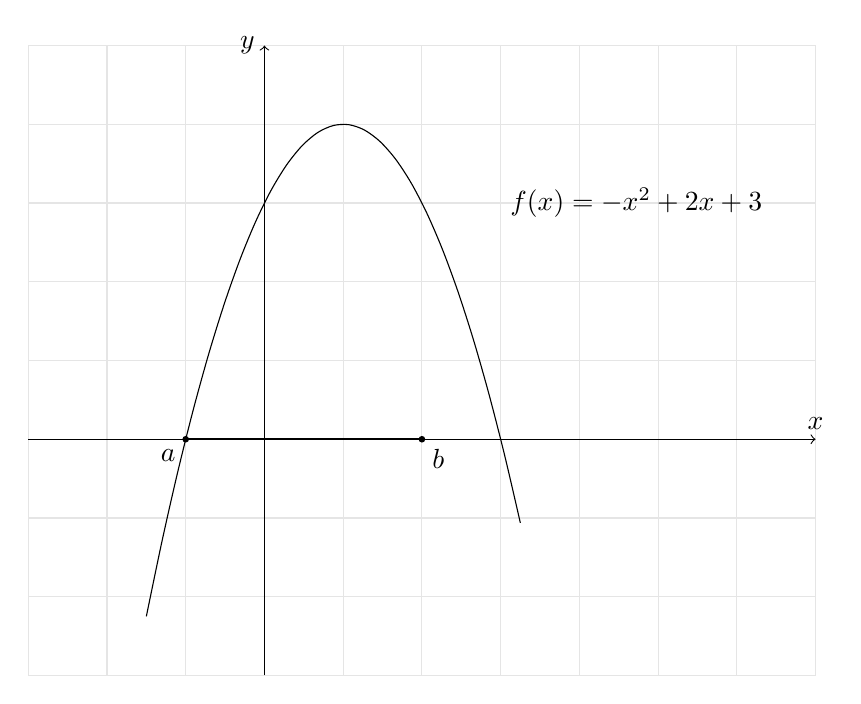
\begin{tikzpicture}
            \draw[gray!20] (-3, -3) grid (7, 5);

            \draw[smooth,domain=-1.5:3.25] plot (\x, {-\x*\x + 2*\x + 3});
            \node[anchor=west] at (3, 3) { $f(x) = -x^2 + 2x + 3$ };

            \draw[->] (0,-3) -- (0, 5) node[anchor=east] { $y$ };
            \draw[->] (-3,0) -- (7, 0) node[anchor=south] { $x$ };

            \draw[thick] (-1, 0) node[anchor=north east] { $a$ } -- (2, 0) node[anchor=north west] { $b$ };

            \fill (-1,0) circle [radius=1.2pt];
            \fill (2,0) circle [radius=1.2pt];
        \end{tikzpicture}
    \end{figure}

\end{frame}

\begin{frame}[fragile]{Exemplos de funções unimodais}

    \begin{figure}
        \centering

        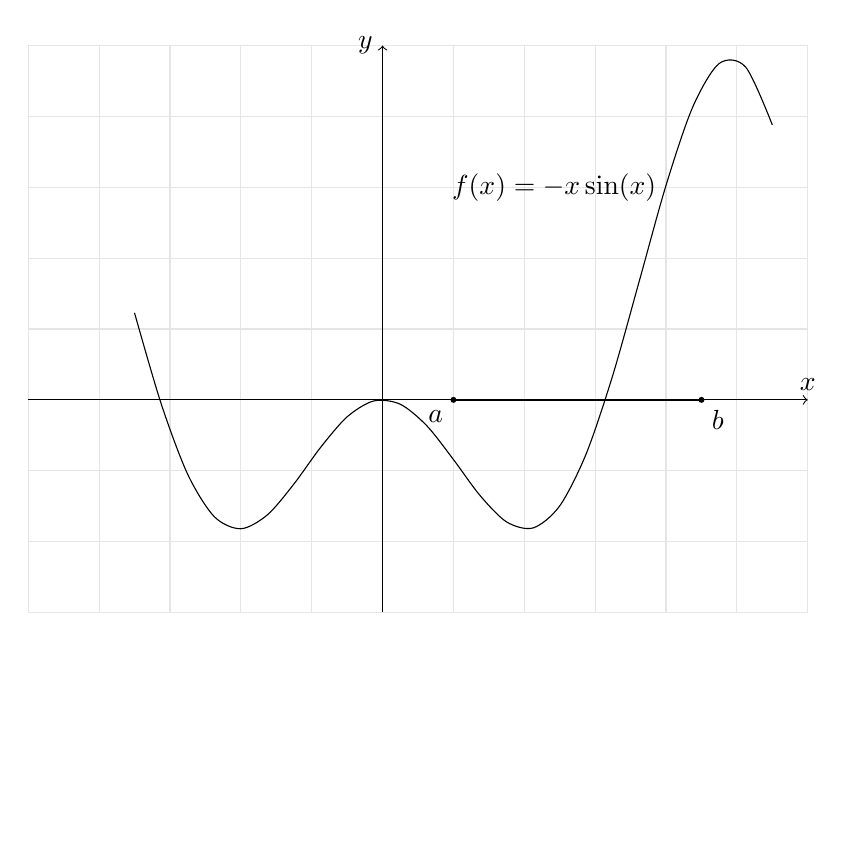
\begin{tikzpicture}
            \begin{scope}[scale=0.9]
                \draw[gray!20] (-5, -3) grid (6, 5);
                \draw[opacity=0] (0,-6);

                \draw[smooth,domain=-3.5:5.5] plot (\x, {-\x*sin(\x r)});
                \node[anchor=east] at (4, 3) { $f(x) = -x\sin(x)$ };

                \draw[->] (0,-3) -- (0, 5) node[anchor=east] { $y$ };
                \draw[->] (-5,0) -- (6, 0) node[anchor=south] { $x$ };

                \draw[thick] (1, 0) node[anchor=north east] { $a$ } -- (4.5, 0) node[anchor=north west] { $b$ };

                \fill (1,0) circle [radius=1.2pt];
                \fill (4.5,0) circle [radius=1.2pt];
            \end{scope}
        \end{tikzpicture}
    \end{figure}

\end{frame}


\begin{frame}[fragile]{Algoritmo}

    \begin{itemize}
        \item Seja $f(x)$ uma função unimodal no intervalo $I = [a, b]$ e $m_1, m_2\in I$ tais
            que $a < m_1 < m_2 < b$, com um valor máximo no ponto $c\in I$

        \item Os valores $f(m_1)$ e $f(m_2)$ se relacionam de uma das três maneiras seguintes:
        \begin{enumerate}
            \item $f(m_1) < f(m_2)$
            \item $f(m_1) > f(m_2)$
            \item $f(m_1) = f(m_2)$
        \end{enumerate}

        \item No primeiro caso, o máximo não pode estar no intervalo $[a, m_1]$, pois 
            área de crescimento da função está à direita de $m_1$

        \item Assim $c > m_1$ e a busca deve prosseguir no intervalo $[m_1, b]$

        \item O segundo caso é simétrico ao primeiro: a região de decrescimento está à 
            esquerda de $m_2$, logo $c$ está no intervalo $[a, m_2]$
    \end{itemize}

\end{frame}

\begin{frame}[fragile]{Algoritmo}

    \begin{itemize}
        \item No terceiro caso ocorre ou quando $m_1 = m_2$ ou se $m_1$ está na área de crescimento
            e $m_2$ na área de decrescimento, ou vice-versa

        \item Assim, $c\in [m_1, m_2]$

        \item Para simplificar o algoritmo, o terceiro caso pode ser reduzido a um dos dois
            primeiros

        \item Se $m_1$ e $m_2$ dividirem $[a, b]$ em três regiões iguais, a cada etapa
            o intervalo de busca é reduzido em um terço de seu tamanho

        \item Para esta divisão os valores a serem escolhidos são
        \begin{align*}
            m_1 &= a + \left(\dfrac{b - a}{3}\right) \\
            m_2 &= b - \left(\dfrac{b - a}{3}\right)
        \end{align*}
    \end{itemize}

\end{frame}

\begin{frame}[fragile]{Exemplos de funções unimodais}

    \begin{figure}
        \centering

        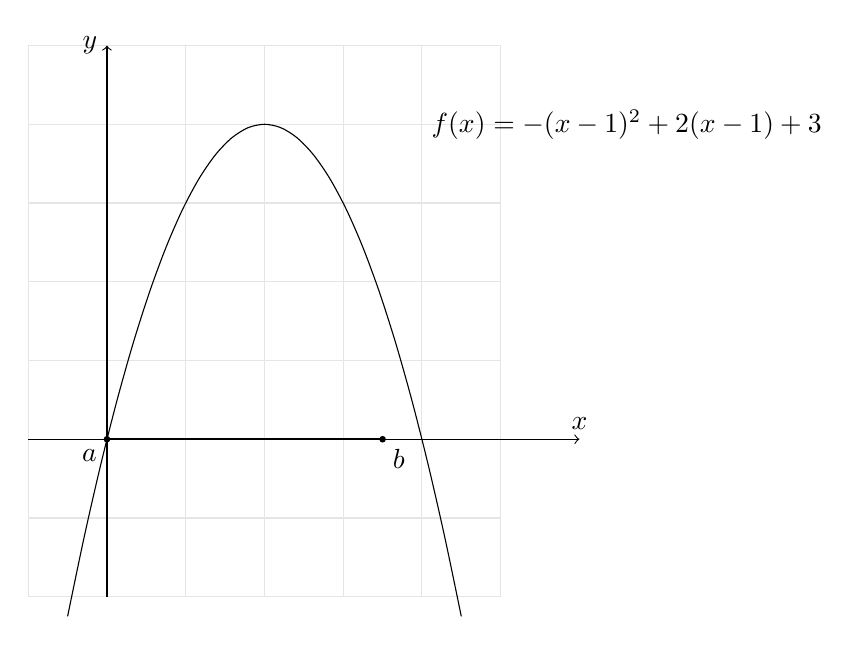
\begin{tikzpicture}
            \draw[gray!20] (-1, -2) grid (5, 5);

            \draw[smooth,domain=-0.5:4.5] plot (\x, {-(\x - 1)*(\x - 1) + 2*(\x - 1) + 3});
            \node[anchor=west] at (4, 4) { $f(x) = -(x - 1)^2 + 2(x - 1) + 3$ };

            \draw[->] (0,-2) -- (0, 5) node[anchor=east] { $y$ };
            \draw[->] (-1,0) -- (6, 0) node[anchor=south] { $x$ };

            \draw[thick] (0, 0) node[anchor=north east] { $a$ } -- (3.5, 0) node[anchor=north west] { $b$ };

            \fill (0,0) circle [radius=1.2pt];
            \fill (3.5,0) circle [radius=1.2pt];
        \end{tikzpicture}
    \end{figure}

\end{frame}

\begin{frame}[fragile]{Exemplos de funções unimodais}

    \begin{figure}
        \centering

        \begin{tikzpicture}
            \draw[gray!20] (-1, -2) grid (5, 5);

            \draw[smooth,domain=-0.5:4.5] plot (\x, {-(\x - 1)*(\x - 1) + 2*(\x - 1) + 3});
            \node[anchor=west] at (4, 4) { $f(x) = -(x - 1)^2 + 2(x - 1) + 3$ };
            \node[anchor=west] at (4, 3.25) { $m_1 = 1.16667, m_2 = 2.33333$ };
            \node[anchor=west] at (4, 2.5) { $f\left(m_1 + \left(\dfrac{m_2 - m_1}{2}\right)\right) = 3.88889$ };

            \draw[->] (0,-2) -- (0, 5) node[anchor=east] { $y$ };
            \draw[->] (-1,0) -- (6, 0) node[anchor=south] { $x$ };

            \draw[dashed] (1.16667, 0) node[anchor=north] { \scriptsize $m_1$ } -- (1.16667, 3.30556);
            \draw[dashed] (2.33333, 0) node[anchor=north] { \scriptsize $m_2$ } -- (2.33333, 3.88889);

\draw[thick] (0, 0) node[anchor=north east] { $a$ } -- (3.5, 0) node[anchor=north west] { $b$ };

            \fill (0,0) circle [radius=1.2pt];
            \fill (3.5,0) circle [radius=1.2pt];
        \end{tikzpicture}
    \end{figure}

\end{frame}

\begin{frame}[fragile]{Exemplos de funções unimodais}

    \begin{figure}
        \centering

        \begin{tikzpicture}
            \draw[gray!20] (-1, -2) grid (5, 5);

            \draw[smooth,domain=-0.5:4.5] plot (\x, {-(\x - 1)*(\x - 1) + 2*(\x - 1) + 3});
            \node[anchor=west] at (4, 4) { $f(x) = -(x - 1)^2 + 2(x - 1) + 3$ };
            \node[anchor=west] at (4, 3.25) { $m_1 = 1.94444, m_2 = 2.72222$ };
            \node[anchor=west] at (4, 2.5) { $f\left(m_1 + \left(\dfrac{m_2 - m_1}{2}\right)\right) = 3.99691$ };

            \draw[->] (0,-2) -- (0, 5) node[anchor=east] { $y$ };
            \draw[->] (-1,0) -- (6, 0) node[anchor=south] { $x$ };

            \draw[dashed] (1.94444, 0) node[anchor=north] { \scriptsize $m_1$ } -- (1.94444, 3.99691);
            \draw[dashed] (2.72222, 0) node[anchor=north] { \scriptsize $m_2$ } -- (2.72222, 3.4784);
            \draw[thick] (1.1667, 0) node[anchor=north east] { $a$ } -- (3.5, 0) node[anchor=north west] { $b$ };

            \fill (1.1667,0) circle [radius=1.2pt];
            \fill (3.5,0) circle [radius=1.2pt];
        \end{tikzpicture}
    \end{figure}

\end{frame}

\begin{frame}[fragile]{Exemplos de funções unimodais}

    \begin{figure}
        \centering

        \begin{tikzpicture}
            \draw[gray!20] (-1, -2) grid (5, 5);

            \draw[smooth,domain=-0.5:4.5] plot (\x, {-(\x - 1)*(\x - 1) + 2*(\x - 1) + 3});
            \node[anchor=west] at (4, 4) { $f(x) = -(x - 1)^2 + 2(x - 1) + 3$ };
            \node[anchor=west] at (4, 3.25) { $m_1 = 1.68519, m_2 = 2.20370$ };
            \node[anchor=west] at (4, 2.5) { $f\left(m_1 + \left(\dfrac{m_2 - m_1}{2}\right)\right) = 3.9585$ };
            \draw[->] (0,-2) -- (0, 5) node[anchor=east] { $y$ };
            \draw[->] (-1,0) -- (6, 0) node[anchor=south] { $x$ };

            \draw[dashed] (1.68519, 0) node[anchor=north] { \scriptsize $m_1$ } -- (1.68519, 3.90089);
            \draw[dashed] (2.20370, 0) node[anchor=north] { \scriptsize $m_2$ } -- (2.20370, 3.9585);
            \draw[thick] (1.1667, 0) node[anchor=north east] { $a$ } -- (2.72222, 0) node[anchor=north west] { $b$ };

            \fill (1.1667,0) circle [radius=1.2pt];
            \fill (2.72222,0) circle [radius=1.2pt];
        \end{tikzpicture}
    \end{figure}

\end{frame}


\begin{frame}[fragile]{Implementação iterativa da busca ternária}
    \inputsnippet{cpp}{1}{19}{codes/ternary.cpp}
\end{frame}

\begin{frame}[fragile]{Implementação recursiva da busca ternária}
    \inputsnippet{cpp}{1}{21}{codes/recursive_ternary.cpp}
\end{frame}
